\documentclass[12pt,a4paper]{article}

\usepackage{amsmath,amsthm,amssymb}
\usepackage[utf8]{vietnam}
\usepackage{blindtext}
\usepackage{listings}
\usepackage{graphicx}
\usepackage[numbers]{natbib}
\usepackage{enumitem}
\renewcommand{\baselinestretch}{1.5}
\begin{document}

%----------------------------------------------------------------------------------------
%	TITLE PAGE
%----------------------------------------------------------------------------------------

\begin{titlepage} % Suppresses displaying the page number on the title page and the subsequent page counts as page 1
	\newcommand{\HRule}{\rule{\linewidth}{0.5mm}} % Defines a new command for horizontal lines, change thickness here
	
	\center % Centre everything on the page
	
	%------------------------------------------------
	%	Headings
	%------------------------------------------------
	
	\textsc{\LARGE đại học khoa học tự nhiên}\\[1.5cm] 
	\textsc{\Large Khoa Toán-tin học}\\[0.5cm] 
	
	\textsc{\large Phương pháp toán trong tin}\\[0.5cm] 
	
	%------------------------------------------------
	%	Title
	%------------------------------------------------
	
	\HRule\\[0.4cm]
	
	{\huge\bfseries Exploiting reinforcement learning to find optimal strategy in dynamic maps}\\[0.4cm] % Title of your document
	
	\HRule\\[1.5cm]
	
	%------------------------------------------------
	%	Author(s)
	%------------------------------------------------
	
	\begin{minipage}{0.4\textwidth}
		\begin{flushleft}
			\large
			\textit{Tác giả}\\
			\textsc{Phan Quang Khánh} % Your name
		\end{flushleft}
	\end{minipage}
	~
	\begin{minipage}{0.4\textwidth}
		\begin{flushright}
			\large
			\textit{Giảng viên hướng dẫn}\\
			TS. Huỳnh Thế \textsc{Đăng} % Supervisor's name
		\end{flushright}
	\end{minipage}
	
	\vfill\vfill\vfill % Position the date 3/4 down the remaining page
	
	{\large\today} % Date, change the \today to a set date if you want to be precise
	
	%------------------------------------------------
	%	Logo
	%------------------------------------------------
	
	%\vfill\vfill
	%\includegraphics[width=0.2\textwidth]{placeholder.jpg}\\[1cm] % Include a department/university logo - this will require the graphicx package
	 
	%----------------------------------------------------------------------------------------
	
	\vfill % Push the date up 1/4 of the remaining page
	
\end{titlepage}
%---------------------------------------------------------------------------------
\clearpage
\tableofcontents
\clearpage
\section{Cơ sở lý thuyết}
\subsection{Q-learning}
Q-learning, trong đó đối tượng trong trò chơi\footnote{agent} tối ưu hàm phần thưởng đặc trưng của trò chơi bằng việc chọn hành động để tối đa hóa hàm tích lũy phần thưởng trong tương lai, là một trong những kỹ thuật mô hình hóa môi trường của agent và tập hành động của nó bằng quá trình quyết định Markov hữu hạn\footnote{finite Markov decision process}.\\
\subsection{SARSA}
\section{Quá trình}
\subsection{Lần thử thứ 1}
\subsubsection{Kết luận}
Agent không ra khỏi vùng an toàn, nghi ngờ rằng vì agent đi trên miền số nguyên mà enemy đi trên miền số thực dẫn đến việc khi tạo state cho model sẽ sinh ra rất nhiếu state. Do đó quá trình exploration của Q- learning sẽ trở nên nặng nề. 
\clearpage
\subsection{Lần thử thứ 2}
\subsubsection{Giả thiết}
Để khắc phục việc quá nhiều state, chúng tôi lấy phần nguyên của vị trí của enemy. Và để agent không ở lại trong vùng an toàn quá lâu, thay đổi trọng số của từng ô trong bản đồ là điều cần thiết.\\
Vì vùng an toàn quá lớn nên chúng tôi cắt giảm bớt bản đồ với kỳ vọng agent sẽ ra vùng nguy hiểm nhiều hơn..
\subsubsection{Thực hiện}
Với reward khi agent ở trên vùng an toàn sẽ bị trừ 1 mỗi lượt và khi trên vùng nguy hiểm sẽ được cộng 1.\\
Cắt giảm bản đồ khi giữ lại chỉ có 2 ô an toàn.\\
\begin{center}
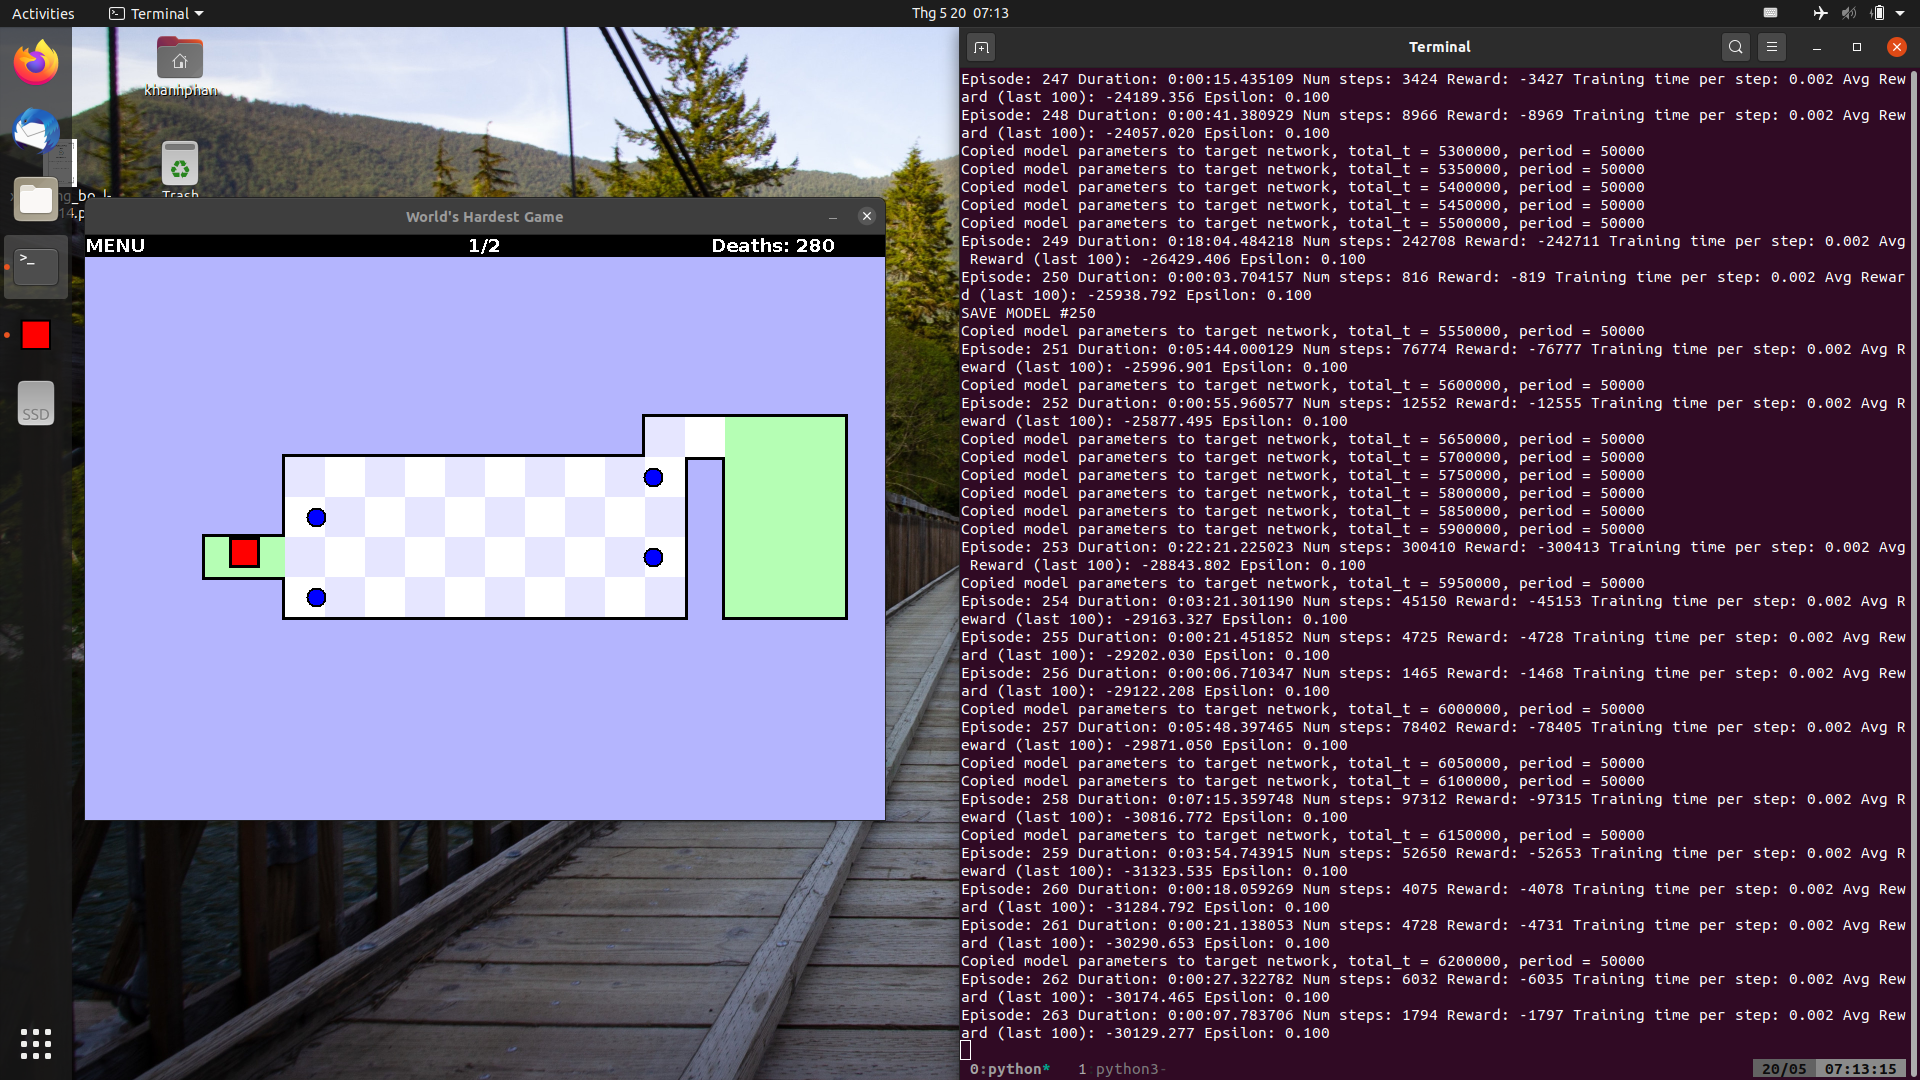
\includegraphics[width=0.95\textwidth]{Thesis_image/try2.png}\\    
\end{center}
Kết quả cho được không được như kỳ vọng sau khoảng 200 episodes, agent nhất quyết không ra khỏi vùng an toàn nữa.
\subsection{Môi trường đơn giản}
Việc đơn giản hóa giúp điều chỉnh model hoạt động 
\begin{center}
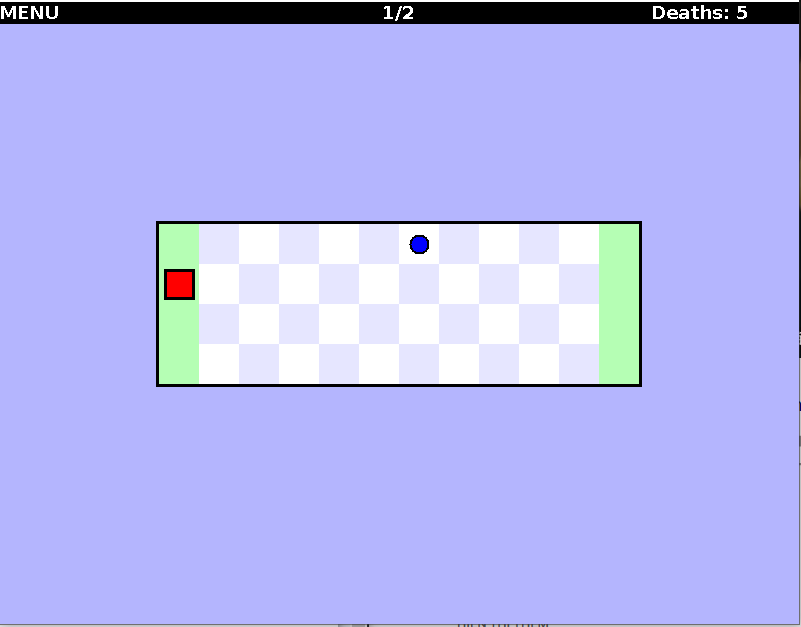
\includegraphics[width=0.95\textwidth]{photo/ThesisRES/1eUp.png}\\    

\end{center}


\end{document}